%%%%%%%%%%%%%%%%%%%%%%%%%%%%%%%%%%%%%%%%%%%%%%%%%%%%%%%%%%%%%%%%%%%%%%%%%%%%%%%%%%%%%%%%%%%
%
%  FORMULARIO ÁREA 2
%
%%%%%%%%%%%%%%%%%%%%%%%%%%%%%%%%%%%%%%%%%%%%%%%%%%%%%%%%%%%%%%%%%%%%%%%%%%%%%%%%%%%%%%%%%%%

\documentclass[10pt]{article}%
\usepackage[latin1]{inputenc}%
\usepackage[brazil]{babel}%
\usepackage{epsfig}%
\usepackage{amsmath}%
\usepackage{amsfonts}%
\usepackage{mathrsfs}%
\usepackage{amssymb}%
\usepackage{graphicx}%
\usepackage{longtable}%
\usepackage{geometry, calc, color, setspace}%
\usepackage{indentfirst}%
\usepackage{wrapfig}%
%\usepackage{cite}
\usepackage[round,authoryear]{natbib}
%\usepackage[colorlinks=true]{hyperref}%
\usepackage{lscape}
\usepackage{booktabs}
%\usepackage{enumitem}

\def\us{\char`\_}

%\pagestyle{empty}

\geometry{a4paper, headsep=1.0cm, footskip=1cm, lmargin=2.5cm, rmargin=2.5cm,
         tmargin=2.5cm, bmargin=2.5cm, headheight=2.5cm}

\renewcommand{\baselinestretch}{1.2}  % Espa\c{c}o entre linhas
\renewcommand{\ra}[1]{\renewcommand{\arraystretch}{#1}}

\def\Var{{\rm Var}\,}
\def\E{{\rm E}\,}
%%%%%%%%%%%%%%%%%%%%%%%%%%%%%%%%%%%%%%%%%%%%%%%%%%%%%%%%%%%%
%
%             In\'{\i}cio do documento
%
%%%%%%%%%%%%%%%%%%%%%%%%%%%%%%%%%%%%%%%%%%%%%%%%%%%%%%%%%%%%
\begin{document}


%%%%%%%%%%%%%%%%%%%%%%%%%%%%%%%%%%%%%%%%%%%%%%%%%%%%%%%%%%%%
\begin{center}
{\bf 
UNIVERSIDADE FEDERAL DO RIO GRANDE DO SUL\\
INSTITUTO DE MATEMÁTICA E ESTATÍSTICA\\
DEPARTAMENTO DE ESTATÍSTICA\\
MAT02219 - PROBABILIDADE E ESTATÍSTICA}\\
\vspace*{0.1cm}{\bf ÁREA 2}
\end{center}
\pagenumbering{arabic}
%%%%%%%%%%%%%%%%%%%%%%%%%%%%%%%%%%%%%%%%%%%%%%%%%%%%%%%%%%%%
%\vspace*{0.1cm}
%\begin{center}
%{\bf INSTRUÇÕES}
%\end{center}
%
%\begin{itemize}%\setlength{\itemsep}{+1mm}
%\item A prova é individual.
%\item A prova é sem consulta, \textbf{com exceção} do formulário que se encontra a seguir.
%\item Você pode utilizar uma calculadora para realizar as questões.
%\begin{itemize}
%\item No caso de uma divisão, você pode deixar o resultado na forma de frações.
%\end{itemize}
%\item Leia com atenção todas as questões antes de resolvê-las.
%\item As questões podem ser realizadas na ordem de sua preferência.
%\item O desenvolvimento das questões será considerado. Portanto, escreva de maneira legível o seu raciocínio, esclarecendo suas suposições para a solução das questões. Não esqueça de indicar claramente o número da questão que você está respondendo.
%\item Coloque o seu nome e número de cartão nas folhas de resolução.
%\item A prova começará as 16 hs 30 min e tem duração de uma hora e quarenta minutos.
%\end{itemize}
%%%%%%%%%%%%%%%%%%%%%%%%%%%%%%%%%%%%%%%%%%%%%%%%%%%%%%%%%%%%
%\newpage
%%%%%%%%%%%%%%%%%%%%%%%%%%%%%%%%%%%%%%%%%%%%%%%%%%%%%%%%%%%%%
%\begin{center}
%{\bf 
%UNIVERSIDADE FEDERAL DO RIO GRANDE DO SUL\\
%INSTITUTO DE MATEMÁTICA E ESTATÍSTICA\\
%DEPARTAMENTO DE ESTATÍSTICA\\
%MAT02219 - PROBABILIDADE E ESTATÍSTICA}\\
%\vspace*{0.5cm}
%{\bf PROVA 2 - 2017/2}
%\end{center}
%%%%%%%%%%%%%%%%%%%%%%%%%%%%%%%%%%%%%%%%%%%%%%%%%%%%%%%%%%%%
%\vspace*{0.5cm}
\begin{center}
{\bf FORMULÁRIO}
\end{center}

%
%\textbf{Tabela de Frequências}
%
%\begin{itemize}%\setlength{\itemsep}{+1mm}
%\item \textbf{Frequências absolutas e relativas:} seja $F_j$ a frequência absoluta do valor/classe $j$ e $n$ o total de elementos do conjunto de dados. A frequência relativa é dada por $f_j = F_j/n$.
%\item \textbf{Número de classes (k):} $k = \sqrt{n}$ (regra empírica); $k = 1 + 3,32 \log{(n)}$, em que $k$ é número de classes e $n$ o número de observações. Ainda, $i = a_t/k$, em que $i$ é a amplitude do intervalo, $a_t = x_{(n)} - x_{(1)}$ é a amplitude total, e $x_{(1)}, x_{(n)}$ são os extremos inferiror e superior do conjunto de dados.
%\end{itemize}
%
%\textbf{Gráficos}
%
%\begin{itemize}
%\item \textbf{Histograma:} a densidade de frequência é dada pela razão entre a frequência relativa da classe e a base (comprimento do intervelo) da classe.
%\end{itemize}
%
%\textbf{Medidas Descritivas}
%
%\emph{Medidas de localização}
%
%\begin{itemize}
%\item \textbf{A média amostral (aritmética simples)} é dada por $\bar{x} = \frac{1}{n}\sum_{i=1}^n{x_i} = \frac{x_1 + x_2 + \ldots + x_n}{n}$.
%\item Suponha que para os dados $x_1, x_2, \ldots, x_n$ possuem os seguintes pesos $p_1, p_2, \ldots, p_n$, então \textbf{a média aritmética ponderada} é dada por $\bar{x}_p = \frac{\sum_{i=1}^n{x_ip_i}}{\sum_{i=1}^n{p_i}}$.
%\begin{itemize}
%%\item Para dados em grupamentos simples, calcula-se a média do seguinte modo 
%%$$
%%\bar{x} = \frac{\sum_{i=1}{n_ix_i}}{\sum_{i=1}{n_i}} = \sum_{i=1}{x_i\frac{n_i}{\sum_{i=1}{n_i}}} = \sum_{i=1}{x_i\frac{n_i}{n}} = \sum_{i=1}{x_if_i}.
%%$$
%\item A média aritmética para dados \textbf{agrupados por intervalo de classe} é dada por $\bar{x} = \frac{\sum_{j}{c_jF_j}}{n}$ em que, $c_j$ é o ponto médio do intervalo de classe. 
%\end{itemize}
%\item A posição da mediana é dada por $p = \frac{n+1}{2}$. A \textbf{mediana} é dada por $Md = x_{(p)}$, quando $n$ é par, e $Md = [x_{(p_1)} + x_{(p_1)}]/2$, quando $n$ é ímpar. As posições dos \textbf{quartis} são dadas por $p_1 = \frac{n+1}{4}; p_2 = \frac{2(n+1)}{4}; p_3 = \frac{3(n+1)}{4}$, se $n$ é ímpar, e $p_1 = \frac{n+2}{4}; p_2 = \frac{2n+2}{4}; p_3 = \frac{3n+2}{4}$. Os quartis são dados por $Q_i = x_{(p_i)}$. Se $p_i$ não for um número inteiro, então $Q_i = (x_{(\lceil p_i\rceil)} + x_{(\lfloor p_i\rfloor)})/2$, em que $\lceil p_i\rceil, \lfloor p_i\rfloor$ são o menor e o maior inteiro de $p_i$.
%\end{itemize}
%
%\emph{Medidas de variação ou dispersão}
%
%\begin{itemize}
%\item A \textbf{amplitude total} é $a_t = x_{(n)} - x_{(1)}$, em que $x_{(1)}, x_{(n)}$ são os extremos inferiror e superior do conjunto de dados.
%\item A \textbf{variância amostral} é dada por $s^2 = \frac{\sum_{i=1}^n{(x_i - \bar{x})^2}}{n - 1} = \frac{\sum_{i=1}^n{x_i^2} - n\bar{x}^2}{n - 1}$.
%\begin{itemize}
%\item A variância amostral para dados \textbf{agrupados por intervalo de classe} é dada por $s^2 = \frac{\sum_{j}{F_j(c_j - \bar{x})^2}}{n-1}$ em que, $c_j$ é o ponto médio do intervalo de classe.
%%\item Fórmulas alternativas da variância:
%%\begin{itemize}
%%\item Dados não agrupados: 
%%$$
%%s^2 = \frac{\sum_{i=1}^n{x_i^2} - \frac{\left(\sum_{i=1}^n{x_i}\right)^2}{n}}{n - 1}.
%%$$
%%\item Dados simplesmente agrupados 
%%$$
%%s^2 = \frac{\sum_{i=1}{n_ix_i^2} - \frac{\left(\sum_{i=1}{n_ix_i}\right)^2}{\sum_{i=1}{n_i}}}{\sum_{i=1}{n_i} - 1}.
%%$$
%%\end{itemize}
%\end{itemize}
%\item O \textbf{desvio padrão amostral} é igual a raiz quadrada da variância amostral: $s = \sqrt{s^2}$.
%\item O \textbf{coeficiente de varição} é $CV = s/\bar{x}$.
%\end{itemize}
%
%\emph{Medidas de formato}
%
%\begin{itemize}
%\item O \textbf{coeficiente de assimetria} é $a_3=m_3/(m_2\sqrt{m_2})$, em que $m_2 = \sum_{i=1}^n{(x_i - \bar{x})^2}/n$ e $m_3 = \sum_{i=1}^n{(x_i - \bar{x})^3}/n$.
%\item O \textbf{coeficiente de curtose} é $a_4=m_4/(m_2)^2$, em que $m_2 = \sum_{i=1}^n{(x_i - \bar{x})^2}/n$ e $m_4 = \sum_{i=1}^n{(x_i - \bar{x})^4}/n$.
%\end{itemize}
%
%\textbf{Probabilidades}
%
%\emph{Técnicas de contagem}
%
%\begin{itemize}%\setlength{\itemsep}{+1mm}
%\item \textbf{Permutações:} ${\rm P}_n = n!$.
%\item \textbf{Arranjos:} ${\rm A}_n^x = \frac{n!}{(n-x)!}$.
%\item \textbf{Combinações:} ${\rm C}_n^x = \frac{n!}{x!(n-x)!}$.
%\end{itemize}
%
%\begin{figure}[!ht]
%\centering
%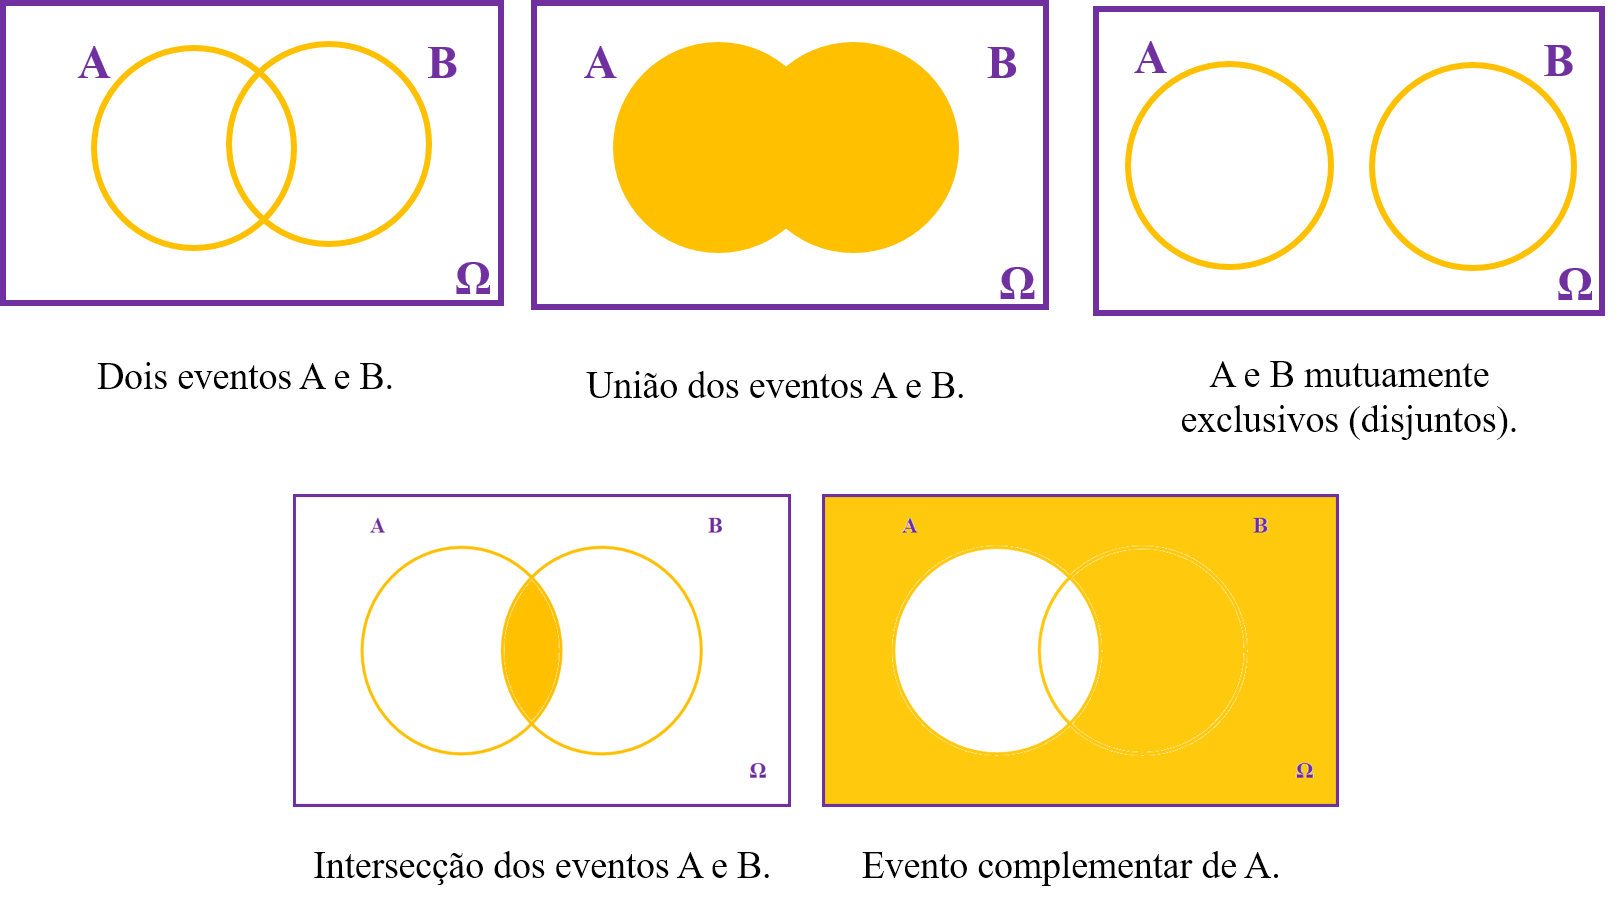
\includegraphics[width=0.8\columnwidth]{eventos_relacoes.png}
%\caption{Operações entre eventos aleatórios.}
%\end{figure}
%
%\emph{Relações entre eventos}
%
%\begin{itemize}%\setlength{\itemsep}{+1mm}
%\item Sejam $A$ e $B$ dois eventos em um espaço amostral $\Omega$. Valem as seguintes relações entre conjuntos:% (De Morgan):
%$$
%\overline{(A\cup B)} = \overline{A} \cap \overline{B}\quad \mbox{e}\quad \overline{(A\cap B)} = \overline{A} \cup \overline{B}.
%$$
%\end{itemize}
%
%\emph{Cálculo de probabilidades}
%
%\begin{itemize}
%\item Regra da adição de probabilidades: sejam $A$ e $B$ eventos em $\Omega$, então $\Pr(A\cup B) = \Pr(A) + \Pr(B) - \Pr(A\cap B)$.
%\item Sejam $A$ e $B$ dois eventos em um espaço amostral $\Omega$. A probabilidade condicional de $B$ dado que o evento $A$ ocorreu é definida como $\Pr(B|A) = \frac{\Pr(A \cap B)}{\Pr(A)},\ \mbox{desde que}\ \Pr(A) > 0$.
%\begin{itemize}
%\item Regra da multiplicação: $\Pr(A \cap B) = \Pr(B|A)\Pr(A)$.
%\item Regra da probabilidade total: consideremos $A$ um evento qualquer referente a $\Omega$, e $B_1, B_2, \ldots, B_k$ uma partição de $\Omega$, então $\Pr(A) = \Pr(A|B_1)\Pr(B_1) + \Pr(A|B_2)\Pr(B_2) + \ldots + \Pr(A|B_k)\Pr(B_k)$.
%\item Teorema de Bayes: seja $B_1, B_2, \ldots, B_k$ uma partição do espaço amostral $\Omega$ e seja $A$ um evento associado a $\Omega$, poderemos escrever
%$$
%\Pr(B_i|A) = \frac{\Pr(A|B_i)\Pr(B_i)}{\Pr(A|B_1)\Pr(B_1) + \Pr(A|B_2)\Pr(B_2) + \ldots + \Pr(A|B_k)\Pr(B_k)}, i = 1, 2, \ldots, k.
%$$
%\end{itemize}
%\end{itemize}
%
%\begin{figure}[ht]
%\centering
%\includegraphics[width=0.25\columnwidth]{keep-calm-and-boa-prova-40.png}
%\end{figure}

\textbf{Variáveis aleatórias}

\begin{itemize}%\setlength{\itemsep}{+1mm}
\item Seja $X$ uma {\bf variável aleatória (v.a.) discreta} ($X$ assume valores em $\{x_1,x_2,\ldots\}$), então o {\bf valor esperado} (média) e a {\bf variância} de $X$, são, respectivamente:
$$
\mu = \E[X] = \sum_{j=1}^{\infty}{x_j p(x_j)}\quad\mbox{e}\quad \sigma^2 = \Var[X] = \E[(X - \mu)^2] = \sum_{j=1}^{\infty}{(x_j - \mu)^2 p(x_j)} = \E[X^2] - \mu^2,
$$
em que $p(x_j) = \Pr(X = x_j)$ é a {\bf função de probabilidade} de $X$ e $\E[X^2] = \sum_{j=1}^{\infty}{x_j^2 p(x_j)}$.
\begin{itemize}
\item[$\bigstar$] Se $X$ {\bf assumir apenas um número finito de valores}, as expressões acima tornam-se $\E[X] = \sum_{j=1}^{n}{x_j p(x_j)}$, $\Var[X] = \sum_{j=1}^{n}{(x_j - \mu)^2 p(x_j)}$ e $\E[X^2] = \sum_{j=1}^{n}{x_j^2 p(x_j)}$.
\end{itemize}
\item Se $X$ é {\bf v.a. contínua}, então o valor esperado (média) e a variância de $X$, são, respectivamente:
$$
\mu = \E[X] = \int_{-\infty}^{\infty}{xf(x)dx}\quad\mbox{e}\quad \sigma^2 = \Var[X] = \E[(X - \mu)^2] = \int_{-\infty}^{\infty}{(x - \mu)^2 f(x)dx} = \E[X^2] - \mu^2,
$$
em que $f(x)$ é a {\bf função densidade de probabilidade} (fdp) de $X$ e $\E[X^2] = \int_{-\infty}^{\infty}{x^2f(x)dx}$.
\begin{itemize}
\item[$\bigstar$] Se $X$ {\bf assumir apenas valores em um intervalo} $S_X \subset \mathbb{R}$, as expressões acima tornam-se $\E[X] = \int_{S_X}{xf(x)dx}$, $\Var[X] = \int_{S_X}{(x - \mu)^2f(x)dx}$ e $\E[X^2] = \int_{S_X}{x^2f(x)dx}$.
\end{itemize}
\item Seja $X$ uma variável aleatória, então $F(x) = \Pr(X\leq x)$ é a {\bf função de distribuição acumulada} (fda) de $X$.
\begin{itemize}
\item[$\bigstar$] $\displaystyle{F(x) = \sum_{j:x_j\leq x}{p(x_j)}}$, se $X$ é v.a. discreta.
\item[$\bigstar$] $\displaystyle{F(x) = \int_{-\infty}^x{f(u)du}}$, se $X$ é v.a. contínua.
\end{itemize}
\end{itemize}

\textbf{Distribuições de probabilidade}

Na Tabela \ref{tab1} considere:
\begin{itemize}
\item ${\rm C}_n^x = {n \choose x} = \frac{n!}{x! (n - x)!}$ é o número de subconjuntos de $x$ elementos diferentes de um conjunto de $n$ elementos diferentes.
\item Para a distribuição Bernoulli e Binomial, $\pi$ representa a probabilidade de sucesso ($\{X = 1\}$).
\item Para as distribuições Normal e $t$-Student, $\pi$ representa o valor $3,14\ldots$.
\item Para as distribuições Qui-quadrado e $t$-Student, $\Gamma(u) = \int_0^{\infty}{x^{u-1}e^{-x}dx}$.
\end{itemize}
\begin{table*}[ht]\centering
\ra{1.3}
\caption{Distribuição de probabilidade, média e variância.}
\label{tab1}
\begin{tabular}{@{}llcc@{}}\toprule
Distribuição de $X$ & $\Pr(X = x)$ & $\E[X]$ & $\Var[X]$\\
\midrule
\multicolumn{4}{c}{\bf Variáveis aleatórias discretas}\\
\midrule
%${\rm Uniforme}(1,k)$ & $\displaystyle{\frac{1}{k}, j = 1, \ldots, k.}$ & $\displaystyle{\frac{1+k}{2}}$ & $\displaystyle{\frac{k^2 - 1}{12}}$\\
%\hline
${\rm Bernoulli}(\pi)$ & $\displaystyle{\pi^x (1 - \pi)^{1 - x}, x = 0,1.}$ & $\pi$ & $\pi(1 - \pi)$\\
\midrule
${\rm Binomial}(n, \pi)$ & $\displaystyle{{n \choose x}\pi^x (1 - \pi)^{n - x}, x = 0,\ldots,n.}$ & $n\pi$ & $n\pi(1 - \pi)$\\
%\midrule
%$\mbox{Geométrica}(p)$ &  $\displaystyle{(1-p)^{j-1}p, j = 1,2,\ldots.}$ & $\displaystyle{\frac{1}{p}}$ & $\displaystyle{\frac{1-p}{p^2}}$\\
\midrule
$\mbox{Hipergeométrica}(n,N,N_1)$ & $\displaystyle{\frac{{\rm C}_{N_1}^x {\rm C}_{N_2}^{n-x}}{{\rm C}_N^n}, x = 0, 1, \ldots, n.}$& $\displaystyle{n\frac{N_1}{N}}$ & $\displaystyle{n\frac{N_1}{N}\frac{N_2}{N}}\left(\frac{N-n}{N-1}\right)$\\
\midrule
${\rm Poisson}(\lambda)$ & $\displaystyle{\frac{e^{-\lambda}\lambda^x}{x!}, x = 0, 1, \ldots.}$& $\lambda$ & $\lambda$\\
\midrule
\multicolumn{4}{c}{\bf Variáveis aleatórias contínuas}\\
\midrule
${\rm Uniforme}(\alpha,\beta)$ & $\displaystyle{\frac{1}{\beta-\alpha}, \alpha\leq x\leq \beta.}$ & $\displaystyle{\frac{\alpha + \beta}{2}}$ & $\displaystyle{\frac{(\beta - \alpha)^2}{12}}$\\
\midrule
${\rm Exponencial}(\lambda)$ &  $\displaystyle{\lambda e^{-\lambda x}, x > 0, \lambda > 0.}$ & $\displaystyle{\frac{1}{\lambda}}$ & $\displaystyle{\frac{1}{\lambda^2}}$\\
\midrule
${\rm Normal}(\mu, \sigma^2)$ & $\displaystyle{\frac{1}{\sqrt{2\pi\sigma^2}}e^{-\frac{(x-\mu)^2}{2\sigma^2}}, -\infty < x < \infty, -\infty < \mu < \infty,  \sigma^2 > 0.}$& $\mu$ & $\sigma^2$\\
\midrule
$\mbox{Normal}(0, 1)$ & $\displaystyle{\frac{1}{\sqrt{2\pi}}e^{-\frac{x^2}{2}}, -\infty < x < \infty.}$& $0$ & $1$\\
\midrule
${\rm Qui-quadrado}(\nu)$ & $\displaystyle{\frac{1}{2^{\nu/2}\Gamma(\nu/2)}x^{\frac{\nu}{x} - 1}e^{\frac{x}{2}}, x \geq 0, \nu > 0.}$& $\nu$ & $2\nu$\\
\midrule
$t{\rm -Student}(\nu)$ & $\displaystyle{\frac{\Gamma((\nu+1)/2)}{\Gamma(\nu/2)\sqrt{\pi\nu}}\left(1+\frac{x^2}{\nu}\right)^{-(\nu+1)/2}, -\infty < x < \infty, \nu > 0.}$& $0$ ($\nu > 1$)& $\frac{\nu}{\nu - 2}$ ($\nu > 2$)\\
\bottomrule
\end{tabular}
\end{table*}

%\begin{table*}[ht]\centering
%\ra{1.3}
%\caption{Variáveis aleatórias contínuas.}
%\begin{tabular}{@{}llcc@{}}\toprule
%Distribuição de $X$ & $f(x)$ & $\E[X]$ & $\Var[X]$\\
%\midrule
%${\rm Uniforme}(\alpha,\beta)$ & $\displaystyle{\frac{1}{\beta-\alpha}, \alpha\leq x\leq \beta.}$ & $\displaystyle{\frac{\alpha + \beta}{2}}$ & $\displaystyle{\frac{(\beta - \alpha)^2}{12}}$\\
%\midrule
%${\rm Exponencial}(\lambda)$ &  $\displaystyle{\lambda e^{-\lambda x}, x > 0, \lambda > 0.}$ & $\displaystyle{\frac{1}{\lambda}}$ & $\displaystyle{\frac{1}{\lambda^2}}$\\
%\midrule
%${\rm Normal}(\mu, \sigma^2)$ & $\displaystyle{\frac{1}{\sqrt{2\pi\sigma^2}}e^{-\frac{(x-\mu)^2}{2\sigma^2}}, -\infty < x < \infty, -\infty < \mu < \infty,  \sigma^2 > 0.}$& $\mu$ & $\sigma^2$\\
%\midrule
%$\mbox{Normal}(0, 1)$ & $\displaystyle{\frac{1}{\sqrt{2\pi}}e^{-\frac{x^2}{2}}, -\infty < x < \infty.}$& $0$ & $1$\\
%\bottomrule
%\end{tabular}
%\end{table*}

\newpage
\textbf{Distribuições amostrais e estimação}

\begin{itemize}
\item Sejam $X_1, X_2, \ldots, X_n$ variáveis aleatórias independentes. A média amostral é dada por 
$$
\bar{X} = \frac{1}{n}\sum_{i=1}^n{X_i} = \sum_{i=1}^n{X_i\frac{1}{n}} = \frac{X_1 + X_2 + \ldots + X_n}{n}.
$$
\begin{itemize}
\item[$\bigstar$] Se $X$ assumir apenas os valores 0 (item não possui determinada característica) ou 1 (item possui determinada característica), então a proporção de itens que possuem a característica na amostra é dada por
$$
p = \frac{\mbox{número de itens com a característica na amostra}}{n}
$$
Note que neste caso $p = \bar{X} = \frac{\sum_{i=1}^n{X_i}}{n}$.
\end{itemize}
\item A variância amostral é dada por:
$$
S^2 = \frac{\sum_{i=1}^n{(X_i - \bar{X})^2}}{n - 1} = \frac{\sum_{i=1}^n{X_i^2} - \frac{\left(\sum_{i=1}^n{X_i}\right)^2}{n}}{n - 1}.
$$
\begin{itemize}
\item[$\bigstar$] O desvio padrão amostral é dado por $S = \sqrt{S^2}$.
\end{itemize}
\item Sejam $X_1, X_2, \ldots, X_n$ variáveis aleatórias independentes com distribuição normal de média $\E[X_i] = \mu$ e variância $\Var[X_i] = \sigma^2$, $i = 1, \ldots, n$, então
$$
\frac{\bar{X} - \mu}{\sigma/\sqrt{n}} \sim N(0,1).
$$
Disso concluímos que $\bar{X}\sim N(\mu,\sigma^2/n)$.
\begin{itemize}
\item[$\bigstar$] Se a variância $\sigma^2$ é desconhecida, então $T = \frac{\bar{X} - \mu}{S/\sqrt{n}} \sim t(\nu)$, com $\nu = n - 1$ ($T$ tem uma distribuição $t$-Student com $\nu$ graus de liberdade).
\item[$\bigstar$] No caso em que a variância é conhecida, a distribuição de $X_i$ não é normal, mas o tamanho da amostra $n$ é grande, então $\bar{X}$ tem distribuição aproximadamente normal ($\frac{\bar{X} - \mu}{\sigma/\sqrt{n}} \approx N(0,1)$).
\item[$\bigstar$] No caso em que a distribuição de $X_i$ não é normal, e seja $Q = \frac{(n-1)S^2}{\sigma^2}$, então $Q\sim \chi^2_{(\nu)}$, com $\nu = n - 1$ ($Q$ tem uma distribuição qui-quadrado com $\nu$ graus de liberdade).
\end{itemize}
\item Seja $Z$ uma variável aleatória com distribuição normal padrão ($Z\sim N(0,1)$), e $\Pr(-z_{\alpha/2} < Z < z_{\alpha/2}) = 1 - \alpha$ o coeficiente de confiança de um Intervalo de Confiança (IC) de $100\times (1-\alpha)\%$.
\item Seja $T$ uma variável aleatória com $t$-Student com $\nu$ graus de liberdade, o coeficiente de confiança de um (IC) de $100\times (1-\alpha)\%$ é dado por e $\Pr(-t_{\alpha/2} < T < t_{\alpha/2}) = 1 - \alpha$.
\end{itemize}


\begin{table*}[ht]\centering
\ra{1.3}
{\footnotesize
\caption{Intervalos de confiança.}
\begin{tabular}{@{}llcc@{}}\toprule
Parâmetro & Variância & IC $100\times (1-\alpha)\%$ & graus de liberdade $(\nu)$\\
\midrule
$\mu$ & CONHECIDA &$\displaystyle{\left[\bar{X} - z_{\alpha/2}\frac{\sigma}{\sqrt{n}};\bar{X} + z_{\alpha/2}\frac{\sigma}{\sqrt{n}}\right]}$ & - \\
\midrule
$\mu$ & DESCONHECIDA & $\displaystyle{\left[\bar{X} - t_{\alpha/2}\frac{S}{\sqrt{n}};\bar{X} + t_{\alpha/2}\frac{S}{\sqrt{n}}\right]}$ & $\nu = n - 1$ \\
\midrule
$\mu_1 - \mu_2$ & DESCONHECIDA & $\displaystyle{\left[\bar{X}_1 - \bar{X}_2 - t_{\alpha/2}\sqrt{\left(\frac{1}{n_1} + \frac{1}{n_2}\right)S^2};\bar{X}_1 - \bar{X}_2 + t_{\alpha/2}\sqrt{\left(\frac{1}{n_1} + \frac{1}{n_2}\right)S^2}\right]}^{\dag}$ & $\nu = (n_1 - 1) + (n_2 - 1)$\\
\midrule
$\sigma^2$ & - & $\displaystyle{\left[\frac{(n-1)S^2}{q_{\alpha/2, n-1}};\frac{(n-1)S^2}{q^{'}_{\alpha/2, n-1}}\right]}$ & $\nu = n - 1$ \\
\midrule
$\pi$ & - &$\displaystyle{\left[p - z_{\alpha/2}\sqrt{\frac{p(1 - p)}{n}};p + z_{\alpha/2}\sqrt{\frac{p(1 - p)}{n}}\right]}$ & - \\
\hline
\multicolumn{4}{l}{$^{\dag} S^2 = \frac{S_1^2(n_1 - 1) + S_2^2(n_2 - 1)}{(n_1 - 1) + (n_2 - 1)}$.}\\
\bottomrule
\end{tabular}
}
\end{table*}

\emph{Dimensionamento de amostra}

\begin{itemize}
\item Considerando o objetivo de construir um IC $100\times (1-\alpha)\%$ para a média $\mu$ da variável $X$, o tamanho da amostra é dado por $n = z_{\alpha/2}^2\times(\sigma^2/d^2)$, em que $d$ corresponde a metade da amplitude do IC.
\item Considerando o objetivo de construir um IC $100\times (1-\alpha)\%$ para a média $\mu$ da variável $X$, variância desconhecida (mas, possivelmente estimada de uma amostra piloto, $S^2$), o tamanho da amostra é dado por $n = t_{\alpha/2}^2\times(S^2/d^2)$, em que $d$ corresponde a metade da amplitude do IC.
\item Considerando o objetivo de construir um IC $100\times (1-\alpha)\%$ para a proporção $\pi$ da variável $X$, o tamanho da amostra é dado por $n = z_{\alpha/2}^2\times(p(1-p)/d^2)$, em que $d$ corresponde a metade da amplitude do IC.
\end{itemize}
\end{document}
